% =============================================================================
% StructureTower — 圏論的視点
% LuaLaTeX 文書
% =============================================================================
\documentclass[a4paper,11pt]{ltjsarticle}

% --- Core packages ---
\usepackage{luatexja-fontspec}
\usepackage{amsmath,amssymb,amsthm}
\usepackage{mathtools}
\usepackage{tikz-cd}
\usepackage{tikz}
\usetikzlibrary{arrows,decorations.markings,positioning,calc}
\usepackage{enumitem}
\usepackage{hyperref}
\usepackage{cleveref}
\usepackage{tcolorbox}
\usepackage{listings}
\usepackage{xcolor}
\usepackage{geometry}
\usepackage{fancyhdr}
\usepackage{float}
\usepackage{booktabs}
\usepackage{array}

% --- Page geometry ---
\geometry{margin=2.5cm, top=3cm, bottom=3cm}

% --- Fonts ---
\setmainjfont{Harano Aji Mincho}[BoldFont=HaranoAjiMincho-Bold]
\setsansjfont{Harano Aji Gothic}[BoldFont=HaranoAjiGothic-Bold]

% --- Colors ---
\definecolor{leanblue}{HTML}{2563EB}
\definecolor{leanbg}{HTML}{F8FAFC}
\definecolor{leancomment}{HTML}{6B7280}
\definecolor{leankeyword}{HTML}{7C3AED}
\definecolor{leanstring}{HTML}{059669}
\definecolor{accentcolor}{HTML}{1E40AF}
\definecolor{theoremcolor}{HTML}{EFF6FF}
\definecolor{definitioncolor}{HTML}{F0FDF4}
\definecolor{remarkcolor}{HTML}{FFF7ED}
\definecolor{exercisecolor}{HTML}{FDF4FF}

% --- Hyperref ---
\hypersetup{
  colorlinks=true,
  linkcolor=accentcolor,
  urlcolor=leanblue,
  citecolor=accentcolor,
  pdftitle={StructureTower 圏論的視点},
  pdfauthor={su},
}

% --- Theorem environments ---
\theoremstyle{definition}
\newtheorem{definition}{定義}[section]
\newtheorem{example}[definition]{例}
\newtheorem{exercise}[definition]{演習}

\theoremstyle{plain}
\newtheorem{theorem}[definition]{定理}
\newtheorem{lemma}[definition]{補題}
\newtheorem{proposition}[definition]{命題}
\newtheorem{corollary}[definition]{系}

\theoremstyle{remark}
\newtheorem{remark}[definition]{注意}

% --- Lean code environment ---
\lstdefinelanguage{lean4}{
  morekeywords={def,theorem,lemma,example,instance,class,structure,
    where,let,in,do,if,then,else,match,with,fun,return,
    import,open,namespace,section,end,variable,
    inductive,abbrev,noncomputable,private,protected,
    sorry,admit,have,show,suffices,calc,by,exact,
    apply,intro,intros,constructor,cases,induction,
    simp,rw,rfl,ext,ring,linarith,omega,norm_num,
    decide,trivial,assumption,contradiction,
    Type,Prop,Sort,Set,true,false,
    rcases,refine,trans,
    attribute,deriving},
  sensitive=true,
  morecomment=[l]{--},
  morecomment=[n]{/-}{-/},
  morestring=[b]",
  literate=
    {->}{{\(\to\)}}2
    {<->}{{\(\leftrightarrow\)}}3
    {<=}{{\(\leq\)}}2
    {>=}{{\(\geq\)}}2,
}

\lstnewenvironment{leancode}[1][]{%
  \lstset{
    language=lean4,
    basicstyle=\ttfamily\footnotesize,
    keywordstyle=\color{leankeyword}\bfseries,
    commentstyle=\color{leancomment}\itshape,
    stringstyle=\color{leanstring},
    backgroundcolor=\color{leanbg},
    frame=single,
    rulecolor=\color{leanblue!30},
    framesep=8pt,
    xleftmargin=12pt,
    xrightmargin=12pt,
    breaklines=true,
    breakatwhitespace=true,
    showstringspaces=false,
    tabsize=2,
    captionpos=b,
    numbers=left,
    numberstyle=\tiny\color{leancomment},
    numbersep=8pt,
    aboveskip=1em,
    belowskip=1em,
    inputencoding=utf8,
    extendedchars=true,
    #1
  }%
}{}

% --- Tcolorbox styles ---
\tcbuselibrary{skins,breakable}

\newtcolorbox{proofstrategy}{
  colback=remarkcolor,
  colframe=orange!60!black,
  title={\textbf{証明戦略}},
  fonttitle=\sffamily,
  boxrule=0.5pt,
  arc=3pt,
}

\newtcolorbox{mathinsight}{
  colback=theoremcolor,
  colframe=accentcolor,
  title={\textbf{数学的洞察}},
  fonttitle=\sffamily,
  boxrule=0.5pt,
  arc=3pt,
}

\newtcolorbox{exercisebox}{
  colback=exercisecolor,
  colframe=purple!60!black,
  title={\textbf{演習問題}},
  fonttitle=\sffamily,
  boxrule=0.5pt,
  arc=3pt,
}

% --- Header/Footer ---
\pagestyle{fancy}
\fancyhf{}
\renewcommand{\headrulewidth}{0.4pt}
\fancyhead[L]{\small\sffamily\nouppercase{\leftmark}}
\fancyhead[R]{\small\sffamily StructureTower 圏論的視点}
\fancyfoot[C]{\thepage}

% --- Macros ---
\newcommand{\colonequiv}{\coloneqq}
\newcommand{\Tower}{\mathsf{Tower}}
\newcommand{\Set}{\mathbf{Set}}
\newcommand{\Nat}{\mathrm{Nat}}
\newcommand{\Hom}{\mathrm{Hom}}
\newcommand{\Id}{\mathrm{id}}
\newcommand{\map}{\mathrm{map}}
\newcommand{\comap}{\mathrm{comap}}
\newcommand{\reindex}{\mathrm{reindex}}
\newcommand{\colim}{\mathrm{colim}}
\newcommand{\NatIncl}{\hookrightarrow_{\mathrm{lw}}}
\newcommand{\Fix}{\mathrm{Fix}}
\newcommand{\EMAlg}{\mathrm{EMAlg}}
\newcommand{\Kl}{\mathrm{Kl}}
\newcommand{\EM}{\mathrm{EM}}
\newcommand{\OrderHom}{\mathsf{OrderHom}}

% =============================================================================
\begin{document}

% --- Title ---
\title{%
  {\LARGE\sffamily\bfseries StructureTower の圏論的視点}\\[0.5em]
  {\large\sffamily Lean 4 / Mathlib4 による形式化とその数学的解説}%
}
\author{su}
\date{2026年2月}
\maketitle

% --- AI Disclosure ---
\begin{center}
\small
\textit{AI assistance disclosure:}\\
Lean ソースコードは Claude (Anthropic) で骨格を生成し、
Codex (OpenAI) で修正した。\\
\TeX\ 文書は Claude Code (Anthropic) で生成した。\\
著者による加筆・修正は行っていない。\\
内容の正確性は保証されず、誤りがあれば著者の責任である。
\end{center}

\vspace{1em}

% --- Abstract ---
\begin{abstract}
本稿では,前順序集合 $\iota$ で添字づけられた集合の単調族
$\mathrm{StructureTower}(\iota, \alpha)$
を圏論的に組織化する Lean 4 形式化を解説する.
まず塔の圏 $\Tower(\iota)$ を定義し,その圏の公理(単位律・結合律)を検証する.
次に,同一台上の塔の間の levelwise 包含が自然変換に対応することを示す.
さらに,写像 $f\colon\alpha\to\beta$ に沿う共変関手 $\map(f)$ と反変関手
$\comap(f)$,および前順序の射 $\varphi\colon\iota\to\kappa$ に沿う再添字関手
$\reindex(\varphi)$ を構成し,それらの関手法則を証明する.
極限・余極限の観点からは,塔の levelwise 交叉・合併が積・余積・等化子を与えることを示す.
また,閉包作用素から定まる塔が閉包モナドの構造を持つこと,
そこから Kleisli 圏と Eilenberg--Moore 代数が得られることを論じる.
最後に,$\mathrm{StructureTower}(\iota,\alpha)$ が順序準同型の圏
$\OrderHom(\iota, \mathcal{P}(\alpha))$ と同値であることを示す.
\end{abstract}

\tableofcontents
\newpage

% =============================================================================
\section{序論:塔という構造}
% =============================================================================

数学において,集合の「段階的な拡大列」はいたるところに現れる.
フィルトレーション,閉包系,層の茎,イデアルの増大列……
これらはすべて,ある半順序集合で添字づけられた集合の単調族として統一的に捉えられる.

本稿が扱う \emph{構造塔} $\mathrm{StructureTower}(\iota,\alpha)$ は,
前順序集合 $(\iota, \leq)$ で添字づけられた $\alpha$ の部分集合の族
$\{T_i\}_{i\in\iota}$ であって,$i \leq j \Rightarrow T_i \subseteq T_j$
を満たすものである.この定義は単純に見えるが,圏論的に豊かな構造を持つ.

\begin{itemize}
  \item \textbf{§1}: 塔を対象,レベル保存写像を射とする圏 $\Tower(\iota)$ の公理
  \item \textbf{§2}: levelwise 包含 $\NatIncl$ を自然変換として解釈
  \item \textbf{§3}: $\map$, $\comap$, $\reindex$ という3種の関手的操作
  \item \textbf{§4}: 積・余積・等化子の levelwise 構成と普遍性
  \item \textbf{§5}: 閉包作用素から定まるモナドと Kleisli / EM の理論
  \item \textbf{§6}: $\OrderHom(\iota, \mathcal{P}(\alpha))$ との同値性
\end{itemize}

% =============================================================================
\section{基礎:構造塔と塔の圏}
\label{sec:foundation}
% =============================================================================

\subsection{構造塔の定義}

\begin{definition}[構造塔]
\label{def:structure-tower}
前順序集合 $(\iota,\leq)$ と集合 $\alpha$ を固定する.
\emph{構造塔} $T = (T_i)_{i\in\iota}$ とは,
各 $i\in\iota$ に $\alpha$ の部分集合 $T_i \subseteq \alpha$ を対応させる族であって,
\[
  i \leq j \;\Longrightarrow\; T_i \subseteq T_j
  \qquad (\forall\, i,j\in\iota)
\]
を満たすものである.$\mathrm{StructureTower}(\iota, \alpha)$ でその全体を表す.
\end{definition}

Lean 4 では次のように定義される:

\begin{leancode}
@[ext]
structure StructureTower (iota alpha : Type*) [Preorder iota] : Type _ where
  level          : iota -> Set alpha
  monotone_level : forall {i j : iota}, i <= j -> level i <= level j
\end{leancode}

\begin{figure}[H]
\centering
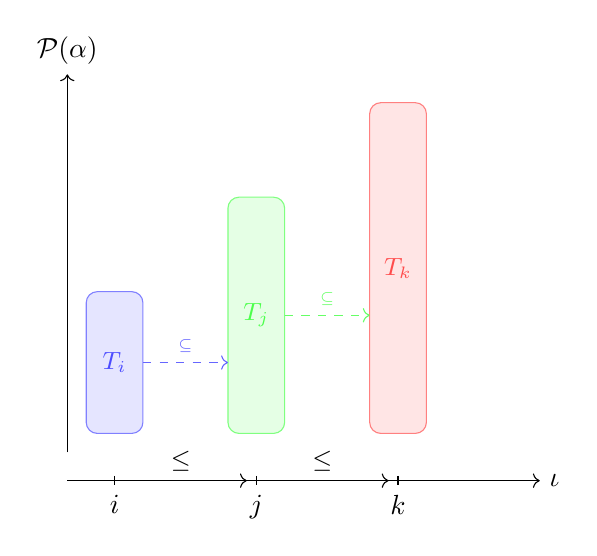
\begin{tikzpicture}[scale=1.2]
  % iota axis
  \draw[->] (0,0) -- (5,0) node[right] {$\iota$};
  \foreach \x/\lab in {0.5/i, 2/j, 3.5/k} {
    \draw (\x,0.05) -- (\x,-0.05) node[below] {$\lab$};
  }
  \draw[->] (0.5,0) -- (1.9,0) node[above,midway,font=\small] {$\leq$};
  \draw[->] (2,0) -- (3.4,0) node[above,midway,font=\small] {$\leq$};
  % Sets
  \draw[fill=blue!10, draw=blue!50, rounded corners] (0.2,0.5) rectangle (0.8,2.0);
  \node[blue!70, font=\small] at (0.5,1.25) {$T_i$};
  \draw[fill=green!10, draw=green!50, rounded corners] (1.7,0.5) rectangle (2.3,3.0);
  \node[green!70, font=\small] at (2.0,1.75) {$T_j$};
  \draw[fill=red!10, draw=red!50, rounded corners] (3.2,0.5) rectangle (3.8,4.0);
  \node[red!70, font=\small] at (3.5,2.25) {$T_k$};
  % Inclusion arrows
  \draw[->, dashed, blue!60] (0.8,1.25) -- (1.7,1.25) node[above,midway,font=\tiny] {$\subseteq$};
  \draw[->, dashed, green!60] (2.3,1.75) -- (3.2,1.75) node[above,midway,font=\tiny] {$\subseteq$};
  % alpha label
  \draw[->] (0,0.3) -- (0,4.3) node[above] {$\mathcal{P}(\alpha)$};
\end{tikzpicture}
\caption{構造塔:$i \leq j \leq k \Rightarrow T_i \subseteq T_j \subseteq T_k$.
  前順序 $\iota$ に沿って部分集合が単調に拡大する.}
\label{fig:structure-tower}
\end{figure}

\subsection{塔の圏 $\Tower(\iota)$}

\begin{definition}[塔の圏]
\label{def:tower-category}
前順序集合 $\iota$ を固定する.\emph{塔の圏} $\Tower(\iota)$ を次で定義する:
\begin{itemize}
  \item \textbf{対象}:型 $\alpha$ が任意に変わる構造塔
    $T \in \mathrm{StructureTower}(\iota, \alpha)$
  \item \textbf{射} $f\colon T_1 \to T_2$($T_1 \in \mathrm{StructureTower}(\iota,\alpha)$,
    $T_2 \in \mathrm{StructureTower}(\iota,\beta)$):
    関数 $f\colon \alpha \to \beta$ であって,各レベルを保存するもの:
    \[
      f(T_{1,i}) \subseteq T_{2,i} \qquad (\forall\, i \in \iota)
    \]
  \item \textbf{恒等射}:$\Id_T = \mathrm{id}_\alpha$
  \item \textbf{合成}:$g \circ f = g_{\mathrm{fun}} \circ f_{\mathrm{fun}}$
\end{itemize}
\end{definition}

\begin{theorem}[圏の公理]
\label{thm:category-axioms}
$\Tower(\iota)$ は以下の圏の公理をすべて満たす:
\begin{enumerate}
  \item \textbf{左単位律}:$\Id \circ f = f$
  \item \textbf{右単位律}:$f \circ \Id = f$
  \item \textbf{結合律}:$(h \circ g) \circ f = h \circ (g \circ f)$
\end{enumerate}
\end{theorem}

\begin{figure}[H]
\centering
\begin{tikzcd}[column sep=4em, row sep=3em]
  T_1 \arrow[r, "f"] \arrow[rr, bend right=20, "g \circ f"']
  & T_2 \arrow[r, "g"]
  & T_3
\end{tikzcd}
\caption{塔の圏における射の合成.関数 $g \circ f\colon \alpha \to \gamma$ は
各レベル $i$ で $f(T_{1,i}) \subseteq T_{2,i}$, $g(T_{2,i}) \subseteq T_{3,i}$
を経由して $g(f(T_{1,i})) \subseteq T_{3,i}$ を満たす.}
\label{fig:composition}
\end{figure}

\begin{proofstrategy}
各公理は関数合成の公理から直接従う.Lean では \texttt{ext} タクティクで
関数の外延的等号に帰着し,\texttt{rfl} で閉じる.
\end{proofstrategy}

% =============================================================================
\section{自然変換としての levelwise 包含}
\label{sec:nat-inclusion}
% =============================================================================

\begin{definition}[NatInclusion / levelwise 包含]
\label{def:nat-inclusion}
同一の前順序 $\iota$ と台集合 $\alpha$ を持つ2つの塔
$T_1, T_2 \in \mathrm{StructureTower}(\iota,\alpha)$ に対して,
\emph{levelwise 包含} $T_1 \NatIncl T_2$ を
\[
  T_1 \NatIncl T_2 \;\colonequiv\; \forall i \in \iota,\; T_{1,i} \subseteq T_{2,i}
\]
で定義する.
\end{definition}

\begin{mathinsight}
各塔は関手 $T\colon (\iota, \leq) \to (\mathcal{P}(\alpha), \subseteq)$ とみなせる.
levelwise 包含 $T_1 \NatIncl T_2$ は,この2つの関手の間の自然変換に他ならない.
\[
\begin{tikzcd}[column sep=3em, row sep=2em]
  (\iota,\leq)
    \arrow[rr, bend left=30, "T_1", ""{name=A, below}]
    \arrow[rr, bend right=30, "T_2"', ""{name=B, above}]
  &&
  (\mathcal{P}(\alpha),\subseteq)
  \arrow[from=A, to=B, Rightarrow, "\eta"]
\end{tikzcd}
\]
自然性条件 $T_{1,i} \subseteq T_{2,i}$($\eta_i$)は Set の射が $\subseteq$ であるため,
自然性図式は自動的に可換になる.
\end{mathinsight}

\begin{proposition}[半順序構造]
\label{prop:partial-order}
同一台 $\alpha$ を持つ塔全体 $\mathrm{StructureTower}(\iota,\alpha)$ の上で,
levelwise 包含は半順序をなす:
\begin{enumerate}
  \item \textbf{反射律}:$T \NatIncl T$
  \item \textbf{推移律}:$T_1 \NatIncl T_2$, $T_2 \NatIncl T_3 \Rightarrow T_1 \NatIncl T_3$
  \item \textbf{反対称律}:$T_1 \NatIncl T_2$, $T_2 \NatIncl T_1 \Rightarrow T_1 = T_2$
\end{enumerate}
\end{proposition}

% =============================================================================
\section{関手的操作:map, comap, reindex}
\label{sec:functors}
% =============================================================================

3種の関手的操作が自然に現れる.

\subsection{共変関手 map}

\begin{definition}[map]
\label{def:map}
関数 $f\colon \alpha \to \beta$ と塔 $T \in \mathrm{StructureTower}(\iota,\alpha)$ に対して,
\[
  \map(f)(T)_i \colonequiv f(T_i) = \{f(x) \mid x \in T_i\}
\]
により塔 $\map(f)(T) \in \mathrm{StructureTower}(\iota,\beta)$ を定義する.
\end{definition}

\begin{definition}[comap]
\label{def:comap}
関数 $f\colon \alpha \to \beta$ と塔 $S \in \mathrm{StructureTower}(\iota,\beta)$ に対して,
\[
  \comap(f)(S)_i \colonequiv f^{-1}(S_i) = \{x \in \alpha \mid f(x) \in S_i\}
\]
により塔 $\comap(f)(S) \in \mathrm{StructureTower}(\iota,\alpha)$ を定義する.
\end{definition}

\begin{definition}[reindex]
\label{def:reindex}
単調写像 $\varphi\colon (\iota,\leq) \to (\kappa,\leq)$ と
塔 $T \in \mathrm{StructureTower}(\kappa,\alpha)$ に対して,
\[
  \reindex(\varphi)(T)_i \colonequiv T_{\varphi(i)}
\]
により塔 $\reindex(\varphi)(T) \in \mathrm{StructureTower}(\iota,\alpha)$ を定義する.
\end{definition}

\begin{figure}[H]
\centering
\begin{tikzcd}[column sep=5em, row sep=3em]
  \mathrm{ST}(\iota,\alpha)
    \arrow[r, "\map(f)", bend left=15]
    \arrow[d, "\reindex(\varphi)"']
  & \mathrm{ST}(\iota,\beta)
    \arrow[l, "\comap(f)", bend left=15]
    \arrow[d, "\reindex(\varphi)"] \\
  \mathrm{ST}(\kappa,\alpha)
    \arrow[r, "\map(f)"', bend right=15]
  & \mathrm{ST}(\kappa,\beta)
    \arrow[l, "\comap(f)"', bend right=15]
\end{tikzcd}
\caption{3種の関手的操作の関係.$\map(f)$ と $\reindex(\varphi)$ は可換
(定理~\ref{thm:map-reindex-comm}).
$\comap(f) \dashv \map(f)$ はここでは随伴ではなく,adjoint-like な性質(命題~\ref{prop:adjoint})を持つ.}
\label{fig:three-functors}
\end{figure}

\begin{theorem}[関手法則]
\label{thm:functor-laws}
\mbox{}
\begin{enumerate}
  \item $\map(\mathrm{id}) = \mathrm{id}$,$\map(g \circ f) = \map(g) \circ \map(f)$
  \item $\comap(\mathrm{id}) = \mathrm{id}$,$\comap(f) \circ \comap(g) = \comap(g \circ f)$
  \item $\reindex(\mathrm{id}) = \mathrm{id}$,$\reindex(g \circ f) = \reindex(f) \circ \reindex(g)$
\end{enumerate}
すなわち $\map$ は共変関手,$\comap$ は反変関手,$\reindex$ は添字の反変関手である.
\end{theorem}

\begin{theorem}[map と reindex の可換性]
\label{thm:map-reindex-comm}
単調写像 $\varphi\colon\iota\to\kappa$,関数 $g\colon\alpha\to\beta$ に対し:
\[
  \map(g) \circ \reindex(\varphi) = \reindex(\varphi) \circ \map(g)
\]
\end{theorem}

\begin{proposition}[map--comap 随伴的関係]
\label{prop:adjoint}
$f\colon\alpha\to\beta$,$T \in \mathrm{ST}(\iota,\alpha)$,$S \in \mathrm{ST}(\iota,\beta)$ に対して:
\[
  \map(f)(T) \NatIncl S
  \;\iff\;
  T \NatIncl \comap(f)(S)
\]
\end{proposition}

\begin{figure}[H]
\centering
\begin{tikzcd}[column sep=6em]
  \mathrm{ST}(\iota,\alpha)
    \arrow[r, bend left=20, "\map(f)"{name=L, above}]
  & \mathrm{ST}(\iota,\beta)
    \arrow[l, bend left=20, "\comap(f)"{name=R, below}]
\end{tikzcd}
\quad $\map(f) \dashv \comap(f)$
\caption{$\map(f) \dashv \comap(f)$:
  $\map(f)(T) \NatIncl S \iff T \NatIncl \comap(f)(S)$.
  前者の「塔の像が $S$ に含まれる」と後者の「塔が $S$ の逆像に含まれる」が同値になる随伴的対応.}
\label{fig:adjunction}
\end{figure}

% =============================================================================
\section{極限・余極限}
\label{sec:limits}
% =============================================================================

同一台 $\alpha$ の塔を対象,$\NatIncl$ を射とする圏を考えると,
この圏は levelwise 集合演算によって豊富な極限・余極限を持つ.

\begin{theorem}[終対象と始対象]
\label{thm:terminal-initial}
\mbox{}
\begin{itemize}
  \item \textbf{終対象}:$\mathbf{1} = (T^{\mathbf{1}}_i \colonequiv \alpha)_{i\in\iota}$
    (各レベルが全集合)は終対象.すなわち任意の $T$ に対して $T \NatIncl \mathbf{1}$.
  \item \textbf{始対象}:$\mathbf{0} = (T^{\mathbf{0}}_i \colonequiv \emptyset)_{i\in\iota}$
    (各レベルが空集合)は始対象.すなわち任意の $T$ に対して $\mathbf{0} \NatIncl T$.
\end{itemize}
\end{theorem}

\subsection{積と余積}

\begin{definition}[積と余積]
\label{def:prod-coprod}
塔 $T_1, T_2 \in \mathrm{StructureTower}(\iota,\alpha)$ に対して:
\begin{align*}
  (T_1 \times T_2)_i &\colonequiv T_{1,i} \cap T_{2,i} \qquad (\text{積}) \\
  (T_1 + T_2)_i &\colonequiv T_{1,i} \cup T_{2,i} \qquad (\text{余積})
\end{align*}
\end{definition}

\begin{theorem}[積の普遍性]
\label{thm:prod-univ}
任意の塔 $S$ に対して,
\[
  S \NatIncl (T_1 \times T_2)
  \;\iff\;
  S \NatIncl T_1 \;\text{ かつ }\; S \NatIncl T_2
\]
\end{theorem}

\begin{figure}[H]
\centering
\begin{tikzcd}[column sep=4em, row sep=3em]
  & S \arrow[dl, "\exists!\,h"'] \arrow[d, dashed] \arrow[dr, "k_2"] & \\
  T_1 & T_1 \times T_2 \arrow[l, "\pi_1"] \arrow[r, "\pi_2"'] & T_2
\end{tikzcd}
\caption{積の普遍性:$S$ から $T_1$ と $T_2$ への $\NatIncl$ の対があれば,
$S \to T_1 \times T_2$ へ一意に因数分解される(ここで矢印は $\NatIncl$).
Lean では \texttt{prod\_univ} として証明済み.}
\label{fig:product-universal}
\end{figure}

\begin{theorem}[余積の普遍性]
\label{thm:coprod-univ}
任意の塔 $S$ に対して,
\[
  (T_1 + T_2) \NatIncl S
  \;\iff\;
  T_1 \NatIncl S \;\text{ かつ }\; T_2 \NatIncl S
\]
\end{theorem}

\begin{figure}[H]
\centering
\begin{tikzcd}[column sep=4em, row sep=3em]
  T_1 \arrow[r, "\iota_1"] \arrow[dr, "h_1"'] & T_1 + T_2 \arrow[d, dashed, "\exists!\,h"] & T_2 \arrow[l, "\iota_2"'] \arrow[dl, "h_2"] \\
  & S &
\end{tikzcd}
\caption{余積の普遍性:$T_1$ と $T_2$ から $S$ への $\NatIncl$ の対があれば,
$T_1 + T_2 \to S$ へ一意に因数分解される.}
\label{fig:coproduct-universal}
\end{figure}

\subsection{無限積・余積}

\begin{definition}[indexed iInf / iSup]
\label{def:iinf-isup}
族 $(T_s)_{s\in\sigma}$($\sigma$ は任意の型)に対して:
\begin{align*}
  \left(\bigwedge_{s\in\sigma} T_s\right)_i &\colonequiv \bigcap_{s\in\sigma} (T_s)_i \\
  \left(\bigvee_{s\in\sigma} T_s\right)_i &\colonequiv \bigcup_{s\in\sigma} (T_s)_i
\end{align*}
\end{definition}

\begin{proposition}
\label{prop:prod-as-iinf}
$T_1 \times T_2 = \bigwedge_{b\in\mathbf{2}} (b \,?\, T_1 \,:\, T_2)$,
すなわち積は 2 元族の $\mathrm{iInf}$ の特殊例である.
\end{proposition}

\subsection{等化子}

\begin{definition}[等化子]
\label{def:equalizer}
同一台の塔間における等化子は,積と一致する:
\[
  \mathrm{eq}(T_1, T_2) \colonequiv T_1 \times T_2
\]
\end{definition}

\begin{remark}
同一台の場合,$\NatIncl$ の射は集合の包含であるため,
等化子は積(levelwise 交叉)と等しくなる.
一般の圏論的等化子は射の等化を表すが,ここでは特殊化した状況にある.
\end{remark}

\begin{figure}[H]
\centering
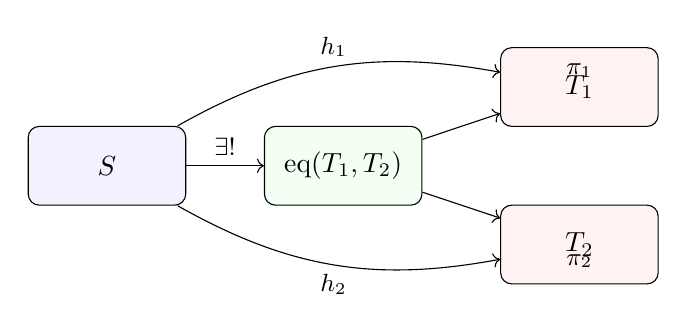
\begin{tikzpicture}[scale=1.0]
  \node[draw, rounded corners, fill=blue!5, minimum width=2cm, minimum height=1cm]
    (S) at (0,0) {$S$};
  \node[draw, rounded corners, fill=green!5, minimum width=2cm, minimum height=1cm]
    (eq) at (3,0) {$\mathrm{eq}(T_1,T_2)$};
  \node[draw, rounded corners, fill=red!5, minimum width=2cm, minimum height=1cm]
    (T1) at (6,1) {$T_1$};
  \node[draw, rounded corners, fill=red!5, minimum width=2cm, minimum height=1cm]
    (T2) at (6,-1) {$T_2$};
  \draw[->] (S) -- (eq) node[above,midway,font=\small] {$\exists!$};
  \draw[->] (eq) -- (T1) node[above,sloped,font=\small] {$\pi_1$};
  \draw[->] (eq) -- (T2) node[below,sloped,font=\small] {$\pi_2$};
  \draw[->, bend left=20] (S) to node[above,font=\small] {$h_1$} (T1);
  \draw[->, bend right=20] (S) to node[below,font=\small] {$h_2$} (T2);
\end{tikzpicture}
\caption{等化子の普遍性(同一台では積と一致).}
\label{fig:equalizer}
\end{figure}

% =============================================================================
\section{閉包モナドと Kleisli / Eilenberg--Moore 理論}
\label{sec:monad}
% =============================================================================

\subsection{閉包作用素から定まる塔}

\begin{definition}[閉包作用素の塔]
\label{def:tower-of-closure}
$(\alpha, \leq)$ を半順序集合,$c\colon\alpha\to\alpha$ を閉包作用素とする.
すなわち $c$ は単調,冪等($c \circ c = c$),かつ $\mathrm{id} \leq c$ を満たす.
このとき:
\[
  (T^c)_x \colonequiv \{y \in \alpha \mid y \leq c(x)\} = {\downarrow}\,c(x)
\]
によって塔 $T^c \in \mathrm{StructureTower}(\alpha, \alpha)$ が定まる.
\end{definition}

\begin{theorem}[モナドの公理]
\label{thm:monad-axioms}
$T^c$ において,閉包作用素のモナド構造の公理が成立する:
\begin{enumerate}
  \item \textbf{単位 (unit)}:$x \in (T^c)_x$,すなわち $x \leq c(x)$
  \item \textbf{乗法 (mult)}:$(T^c)_{c(x)} = (T^c)_x$,すなわち $c(c(x)) = c(x)$
\end{enumerate}
\end{theorem}

\begin{figure}[H]
\centering
\begin{tikzcd}[column sep=5em, row sep=4em]
  T^c \arrow[r, "\eta"] \arrow[dr, "\mathrm{id}"'] & T^c \circ T^c \arrow[d, "\mu"] \\
  & T^c
\end{tikzcd}
\qquad
\begin{tikzcd}[column sep=5em, row sep=4em]
  T^c \circ T^c \arrow[r, "T^c \eta"] \arrow[d, "\mu"'] & T^c \circ T^c \circ T^c \arrow[d, "\mu_{T^c}"] \\
  T^c \arrow[r, "\mu"'] & T^c \circ T^c
\end{tikzcd}
\caption{モナドの公理図式(単位律と結合律).
  $\eta\colon x \mapsto c(x)$(unit),$\mu\colon c(c(x)) = c(x)$(idempotency / mult).}
\label{fig:monad-axioms}
\end{figure}

\subsection{Galois 接続からの構成}

\begin{definition}[Galois 接続の塔]
\label{def:tower-of-galois}
$l\colon\alpha\to\beta$, $u\colon\beta\to\alpha$ が Galois 接続
$l \dashv u$($l(x) \leq y \iff x \leq u(y)$)を形成するとき,
$c_{l,u} \colonequiv u \circ l$ は閉包作用素となる.このとき:
\[
  T^{l,u} \colonequiv T^{c_{l,u}}
\]
\end{definition}

\begin{figure}[H]
\centering
\begin{tikzcd}[column sep=5em, row sep=2em]
  (\alpha, \leq)
    \arrow[r, bend left=25, "l"{above}]
  & (\beta, \leq)
    \arrow[l, bend left=25, "u"{below}]
\end{tikzcd}
\quad ($l \dashv u$)
\qquad
$\Longrightarrow$
\qquad
$c = u \circ l$(閉包作用素)
\caption{Galois 接続 $l \dashv u$ から閉包作用素 $c = u \circ l$ が定まり,
それが塔 $T^{l,u}$ を決定する.}
\label{fig:galois}
\end{figure}

\subsection{Kleisli 圏}

\begin{definition}[Kleisli 圏]
\label{def:kleisli}
閉包作用素 $c$ に対して,\emph{Kleisli 圏} $\Kl(c)$ を次で定義する:
\begin{itemize}
  \item \textbf{対象}:$\alpha$ の元 $x$
  \item \textbf{射} $x \to_{\Kl} y$:$x \leq c(y)$ が成立することを表す命題
  \item \textbf{恒等射}:$x \to_{\Kl} x$($x \leq c(x)$,unit から)
  \item \textbf{合成}:$x \to_{\Kl} y$, $y \to_{\Kl} z$ ならば
    $x \leq c(y) \leq c(c(z)) = c(z)$,ゆえに $x \to_{\Kl} z$
\end{itemize}
直感的に,$x \to_{\Kl} y$ は「$x$ が $c$ の近似・飽和の意味で $y$ に到達可能」を意味する.
\end{definition}

\begin{figure}[H]
\centering
\begin{tikzcd}[column sep=4em, row sep=3em]
  x
    \arrow[r, "{\leq c(y)}"]
    \arrow[rr, bend right=20, "{\leq c(z)}"']
  & y \arrow[r, "{\leq c(z)}"]
  & z
\end{tikzcd}
\caption{Kleisli 圏における射の合成:
$x \leq c(y)$ と $y \leq c(z)$ から $c(y) \leq c(c(z)) = c(z)$ を経て $x \leq c(z)$.
閉包作用素の冪等性が本質的に使われる.}
\label{fig:kleisli-composition}
\end{figure}

\subsection{Eilenberg--Moore 代数}

\begin{definition}[EM 代数]
\label{def:em-algebras}
$x \in \alpha$ が \emph{Eilenberg--Moore 代数}(または \emph{閉元})であるとは,
\[
  c(x) \leq x
\]
が成立することをいう.$\EMAlg(c) \colonequiv \{x \in \alpha \mid c(x) \leq x\}$.
\end{definition}

\begin{theorem}[閉元の特徴付け]
\label{thm:em-characterization}
\[
  x \in \EMAlg(c) \;\iff\; c(x) = x
\]
すなわち EM 代数全体は $c$ の不動点集合 $\Fix(c)$ と一致する.
\end{theorem}

\begin{proof}
$c(x) \leq x$ と $x \leq c(x)$(unit 条件)を合わせれば $c(x) = x$.
逆に $c(x) = x$ ならば $c(x) \leq x$ は自明.
\end{proof}

\begin{figure}[H]
\centering
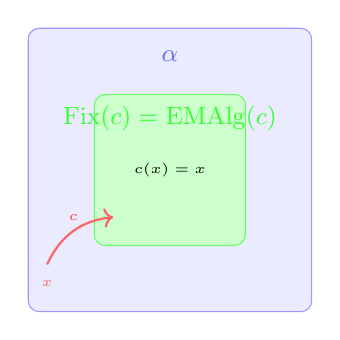
\begin{tikzpicture}[scale=1.2]
  \draw[fill=blue!8, draw=blue!40, rounded corners] (-1.5,-1.5) rectangle (1.5,1.5);
  \node[blue!60, font=\small] at (0, 1.2) {$\alpha$};
  \draw[fill=green!20, draw=green!60, rounded corners] (-0.8,-0.8) rectangle (0.8,0.8);
  \node[green!80, font=\small] at (0, 0.55) {$\Fix(c) = \EMAlg(c)$};
  \node[font=\tiny] at (0, 0) {$c(x) = x$};
  % arrow from outside showing c maps to inside
  \draw[->, thick, red!60] (-1.3, -1.0) to[bend left=30] node[above,font=\tiny,red!80] {$c$} (-0.6,-0.5);
  \node[red!60, font=\tiny] at (-1.3,-1.2) {$x$};
\end{tikzpicture}
\caption{$c\colon\alpha\to\alpha$ は任意の $x$ を不動点集合 $\Fix(c)$ に写す.
  $\EMAlg(c) = \Fix(c)$ であり,EM 代数は $c$ の "安定点" の集合.}
\label{fig:em-algebras}
\end{figure}

% =============================================================================
\section{OrderHom との同値}
\label{sec:orderhom}
% =============================================================================

\begin{theorem}[OrderHom との同値]
\label{thm:orderhom-equiv}
以下の2つの写像:
\begin{align*}
  \Phi\colon \mathrm{StructureTower}(\iota,\alpha) &\to \OrderHom(\iota, \mathcal{P}(\alpha)) \\
  T &\mapsto (i \mapsto T_i) \\[1em]
  \Psi\colon \OrderHom(\iota, \mathcal{P}(\alpha)) &\to \mathrm{StructureTower}(\iota,\alpha) \\
  h &\mapsto (h_i)_{i\in\iota}
\end{align*}
は互いに逆であり,$\Phi \circ \Psi = \mathrm{id}$, $\Psi \circ \Phi = \mathrm{id}$ が成立する.
したがって,
\[
  \mathrm{StructureTower}(\iota,\alpha) \;\simeq\; \OrderHom(\iota, \mathcal{P}(\alpha))
\]
\end{theorem}

\begin{figure}[H]
\centering
\begin{tikzcd}[column sep=6em, row sep=4em]
  \mathrm{StructureTower}(\iota,\alpha)
    \arrow[r, bend left=20, "\Phi"]
    \arrow[loop left, "\mathrm{id}"]
  & \OrderHom(\iota,\mathcal{P}(\alpha))
    \arrow[l, bend left=20, "\Psi"]
    \arrow[loop right, "\mathrm{id}"]
\end{tikzcd}
\caption{StructureTower と OrderHom の同値.$\Phi \circ \Psi = \mathrm{id}$ かつ
$\Psi \circ \Phi = \mathrm{id}$.}
\label{fig:equivalence}
\end{figure}

\begin{proposition}[NatInclusion の OrderHom 的解釈]
\label{prop:nat-orderhom}
$T_1 \NatIncl T_2 \iff \Phi(T_1) \leq \Phi(T_2)$($\OrderHom$ の点状順序)
\end{proposition}

\begin{mathinsight}
この同値は「StructureTower が OrderHom よりも豊かな構造を持つか?」という問いへの答えを与える.
純粋な集合論的意味では両者は同じである.
しかし §3–§5 で構成した $\map$, $\comap$, $\reindex$,
そして閉包モナドの構造は,OrderHom の言葉では表現しにくい代数的制約を明示化している.
\end{mathinsight}

% =============================================================================
\section{演習問題(Lean 4 形式化より)}
\label{sec:exercises}
% =============================================================================

以下は Lean 4 ファイルの §7 に対応する演習問題の数学的解説である.
難易度は 🟢(易)/ 🟡(中)/ 🔴(難)で示す.

\subsection*{Group A:定義の展開}

\begin{exercisebox}
\textbf{A1 🟢 map から Hom を構成せよ}

$f\colon\alpha\to\beta$ と $T \in \mathrm{ST}(\iota,\alpha)$ に対して,
$\Hom(T, \map(f)(T))$ の元を構成せよ.

\textit{ヒント}:射の台関数は $f$ 自身.保存条件は $f(x) \in f(T_i)$ という定義から直接.
\end{exercisebox}

\begin{exercisebox}
\textbf{A3 🟢 iInf の射影}

$S \NatIncl \bigwedge_{s\in\sigma} T_s$ から $S \NatIncl T_{s_0}$(固定 $s_0\in\sigma$)を示せ.

\textit{ヒント}:$\bigwedge$ の定義より $x \in \bigcap_s (T_s)_i \Rightarrow x \in (T_{s_0})_i$.
\end{exercisebox}

\subsection*{Group B:補題の組み合わせ}

\begin{exercisebox}
\textbf{B1 🟡 map--comap 随伴}

$\map(f)(T) \NatIncl S \iff T \NatIncl \comap(f)(S)$ を証明せよ(命題~\ref{prop:adjoint}).

\textit{核心}:
\begin{align*}
(\to)&: x \in T_i \Rightarrow f(x) \in \map(f)(T)_i \subseteq S_i \Rightarrow x \in f^{-1}(S_i) \\
(\leftarrow)&: y \in \map(f)(T)_i \Rightarrow y=f(x),\, x\in T_i \Rightarrow
  x\in\comap(f)(S)_i \Rightarrow f(x)\in S_i
\end{align*}
\end{exercisebox}

\begin{exercisebox}
\textbf{B3 🟡 Kleisli 合成の結合律}

$x \to_{\Kl} y$, $y \to_{\Kl} z$, $z \to_{\Kl} w$ ならば $x \to_{\Kl} w$ を示せ.

\textit{核心}:$\mathtt{kleisli\_comp}$ を2回適用する.
$x \leq c(y)$, $y \leq c(z)$ から $x \leq c(z)$(1回目),
さらに $z \leq c(w)$ と合わせて $x \leq c(w)$(2回目).
\end{exercisebox}

\subsection*{Group C:圏論的推論}

\begin{exercisebox}
\textbf{C1 🔴 map の Hom への作用}

$g\colon\Hom(T_1, T_2)$ と $\beta$ 上の関数 $g_\beta\colon\beta\to\beta$
であって $g_\beta \circ f = f \circ g$ を満たすものが与えられたとき,
$\Hom(\map(f)(T_1), \map(f)(T_2))$ の元を構成せよ.

この構成は関手 $\map(f)\colon\Tower(\iota)\to\Tower(\iota)$ の射への作用に対応する:
\[
\begin{tikzcd}[column sep=4em, row sep=3em]
  T_1 \arrow[r, "g"] \arrow[d, "\map(f)"'] & T_2 \arrow[d, "\map(f)"] \\
  \map(f)(T_1) \arrow[r, dashed, "\exists\,h"] & \map(f)(T_2)
\end{tikzcd}
\]
\end{exercisebox}

\begin{exercisebox}
\textbf{C4 🔴 Galois 接続の単調性と NatInclusion}

$l_1, l_2\colon\alpha\to\beta$ と $u_1, u_2\colon\beta\to\alpha$ が
それぞれ Galois 接続 $l_k \dashv u_k$ を形成し,
$l_1(x) \leq l_2(x)$($\forall x$)かつ $u_1(y) \leq u_2(y)$($\forall y$)が
成り立つとき,$T^{l_1,u_1} \NatIncl T^{l_2,u_2}$ を示せ.

\textit{核心}:
$y \leq u_1(l_1(x))$ を仮定して $y \leq u_2(l_2(x))$ を示す.
$u_1(l_1(x)) \leq u_2(l_2(x))$ は $u_1 \leq u_2$ と $u_2$ の単調性から:
\[
  u_1(l_1(x)) \leq u_2(l_1(x)) \leq u_2(l_2(x))
\]
\end{exercisebox}

% =============================================================================
\section{まとめ}
\label{sec:conclusion}
% =============================================================================

本稿では,構造塔 $\mathrm{StructureTower}(\iota,\alpha)$ の圏論的構造を Lean 4 形式化をもとに解説した.

\begin{table}[H]
\centering
\small
\begin{tabular}{lll}
\toprule
\textbf{概念} & \textbf{数学的内容} & \textbf{Lean の定義名} \\
\midrule
対象の圏 & $\Tower(\iota)$:レベル保存写像 & \texttt{Hom} \\
自然変換 & levelwise 包含 $\NatIncl$ & \texttt{NatInclusion} \\
共変関手 & $\map(f)\colon \mathrm{ST}(\iota,\alpha)\to\mathrm{ST}(\iota,\beta)$ & \texttt{map} \\
反変関手 & $\comap(f)\colon \mathrm{ST}(\iota,\beta)\to\mathrm{ST}(\iota,\alpha)$ & \texttt{comap} \\
再添字関手 & $\reindex(\varphi)\colon \mathrm{ST}(\kappa,\alpha)\to\mathrm{ST}(\iota,\alpha)$ & \texttt{reindex} \\
積 & levelwise 交叉 $T_{1,i}\cap T_{2,i}$ & \texttt{prod} \\
余積 & levelwise 合併 $T_{1,i}\cup T_{2,i}$ & \texttt{coprod} \\
終対象 & 全集合の定数塔 & \texttt{terminal} \\
始対象 & 空集合の定数塔 & \texttt{initial} \\
閉包モナド & $c$ による塔 $T^c_x = {\downarrow}\,c(x)$ & \texttt{towerOfClosure} \\
Kleisli 圏 & 射 $x \to_{\Kl} y \colonequiv x \leq c(y)$ & \texttt{IsKleisliArrow} \\
EM 代数 & $\Fix(c) = \{x \mid c(x) = x\}$ & \texttt{EMAlgebras} \\
同値 & $\mathrm{ST}(\iota,\alpha) \simeq \OrderHom(\iota,\mathcal{P}(\alpha))$ & \texttt{toOrderHom} / \texttt{ofOrderHom} \\
\bottomrule
\end{tabular}
\caption{本稿で扱った主要概念の対応表}
\label{tab:summary}
\end{table}

\begin{mathinsight}
levelwise という操作の原理は徹底している:交叉, 合併, 像, 逆像, 再添字――
すべてが「各レベル $i$ で独立に行い,単調性を継承する」というパターンに従う.
この一貫性が Lean の証明を単純に保ち,圏論的直観を形式化の中に透明に映し出している.
\end{mathinsight}

% =============================================================================
\end{document}
